\documentclass[12pt, a4paper, oneside]{report}
\usepackage[margin=0.9in, top=0.9in, bottom=0.9in]{geometry}
\usepackage[utf8]{inputenc}
\usepackage[T1]{fontenc}
\usepackage{lmodern}
\usepackage{amsmath, amssymb}
\usepackage{booktabs}
\usepackage{array}
\usepackage{tabularx}
\usepackage{fancyhdr}
\usepackage{float}
\usepackage{graphicx}
\usepackage{xcolor}
\usepackage{enumitem}
\usepackage{titlesec}
\usepackage{hyperref}
\usepackage{tikz}
\usetikzlibrary{arrows.meta, positioning}
\tikzset{
  blk/.style={rectangle, rounded corners=4pt, line width=0.8pt, align=center,
              font=\sffamily\small, inner sep=5pt},
  blueb/.style={blk, draw=blue!70!black, fill=blue!6},
  tealb/.style={blk, draw=teal!70!black, fill=teal!6},
  orangeb/.style={blk, draw=orange!80!black, fill=orange!9},
  redb/.style={blk, draw=red!70!black, fill=red!6},
  greenb/.style={blk, draw=green!50!black, fill=green!7},
  pipe/.style={-{Stealth[length=2.4mm]}, line width=0.8pt, draw=black!80},
  steplbl/.style={font=\sffamily\scriptsize\bfseries, fill=white, draw=black!25,
                  line width=0.4pt, inner sep=2pt, rounded corners=1.5pt},
}

\graphicspath{{figures/}}
\setlist{itemsep=2pt, topsep=4pt}
\setlength{\emergencystretch}{2em}

\titleformat{\chapter}[display]
  {\normalfont\LARGE\bfseries}{\chaptertitlename\ \thechapter}{3pt}{\LARGE}
\titlespacing*{\chapter}{0pt}{-35pt}{12pt}
\titlespacing*{\section}{0pt}{10pt}{4pt}
\titlespacing*{\subsection}{0pt}{7pt}{3pt}

% --- Header and Footer ---
\pagestyle{fancy}
\fancyhf{}
\fancyhead[L]{\small\sffamily UCS503 -- Software Engineering Project}
\fancyhead[R]{\small\sffamily AI Cost Autopilot Prototype Report}
\fancyfoot[C]{\thepage}
\renewcommand{\headrulewidth}{0.4pt}
\fancypagestyle{plain}{\fancyhf{}\fancyfoot[C]{\thepage}\renewcommand{\headrulewidth}{0pt}}

% --- Hyperref Setup ---
\hypersetup{
    colorlinks=true,
    linkcolor=blue!70!black,
    citecolor=teal!70!black,
    urlcolor=blue!60!black,
    pdftitle={AI Cost Autopilot: Prototype Report},
    pdfauthor={},
    pdfsubject={UCS503 Software Engineering Project}
}

\newcommand{\code}[1]{\texttt{#1}}

\begin{document}

% =========================================================================
% TITLE PAGE
% =========================================================================
\begin{titlepage}
    \centering
    \vspace*{0.5cm}

    {\Large\bfseries UCS503 -- Software Engineering Project}\\[0.3cm]
    {\large Academic Year 2026--2027}\\[1.5cm]

    {\Huge\bfseries AI Cost Autopilot}\\[0.4cm]
    {\large\textit{A Compiler-Aware Gateway for Token-Cost Optimisation\\in LLM Coding Agents}}\\[2.0cm]

    {\large\textbf{Submitted by:}}\\[0.3cm]
    \begin{tabular}{lll}
        \textbf{1024240033} & Agampreet Kaur   & \textit{Compiler-Aware Trimmer} \\
        \textbf{1024240012} & Devansh Sharma   & \textit{Semantic Cache} \\
        \textbf{1024240029} & Furmaandeep Kaur & \textit{Autopilot Policy} \\
    \end{tabular}\\[0.5cm]
    {\normalsize Computer Science and Engineering Department (CSED)}\\[1.2cm]

    {\large\textbf{Submitted to:}}\\[0.2cm]
    {\large\textbf{Dr. Jeelani Asif}}\\[0.1cm]
    {\normalsize Department of Computer Science and Engineering}\\[1.2cm]

    {\normalsize Repository: \url{https://github.com/agamlotey/ucs503p-202627-ai-cost-autopilot}}\\[0.15cm]
    {\normalsize Documentation: \url{https://agamlotey.github.io/ucs503p-202627-ai-cost-autopilot/}}

    \vfill
    {\normalsize\textbf{Prototype Stage Report}}\\[0.15cm]
    {\normalsize\textbf{Computer Science and Engineering Department}}\\[0.1cm]
    {\normalsize Thapar Institute of Engineering and Technology, Patiala}\\[0.4cm]
\end{titlepage}

% =========================================================================
% TABLE OF CONTENTS
% =========================================================================
\pagenumbering{roman}
\tableofcontents
\newpage
\pagenumbering{arabic}

% =========================================================================
% CHAPTER 1: INTRODUCTION
% =========================================================================
\chapter{Introduction}

\section{Background and Context}

AI coding agents such as Cursor, Claude Code and Codex are now part of everyday
software development. Every time one of them answers a request, it sends a large
slice of the codebase to a large language model (LLM), and the provider bills for
every input and output token. As teams and codebases grow, this becomes one of the
least predictable lines in an engineering budget. Much of what is sent is not
needed for the task at hand: whole files are included when one function matters,
and the same questions are asked again and again.

Before building anything of our own, we checked that the idea was worth pursuing.
We routed the open-source TestZeus Hercules agent through a proxy built from
\emph{existing} tools (Headroom prompt compression behind a LiteLLM proxy). That
proof of concept used about 25\% fewer tokens and cost about 17\% less per run,
with no change in agent behaviour across repeated runs. These figures belong to
the existing tools, not to our system; they only show that a gateway between an
agent and its model can cut cost without breaking the agent.

The same pattern appears in industry. Databricks describes an AI Gateway that
routes requests across models, compresses context and tunes prompt caching, and
reports more than 30\% lower average task cost from routing and almost 50\% fewer
generated tokens from harness and cache tuning, with no observed loss of
quality~\cite{databricks}. Our project builds this kind of gateway ourselves, and
tests whether a \emph{language-aware} way of shrinking context does better than
generic text compression.

\subsection{Problem Statement}

Coding agents send far more code than a task needs, and they repeat requests. Both
waste money. Generic text compressors reduce tokens but know nothing about code
structure, so they can break the code they compress. There is no standard layer
that reduces this spend while keeping the request correct.

The problem we address is: \textbf{reduce the tokens a coding agent sends to an
LLM, without removing anything the task needs and without producing invalid
code}, using a gateway that the agent can use with no change to its workflow.

\section{Project Objectives}

\begin{enumerate}
    \item Build a gateway that speaks the OpenAI-compatible
          \code{/v1/chat/completions} API, so an agent only has to change its base
          URL to use it.
    \item Build a \textbf{compiler-aware trimmer} that parses the code in a request,
          keeps the functions the task is about together with the functions they
          call, and collapses the rest to signatures, always producing valid code.
    \item Build a \textbf{semantic cache} that returns a stored answer when a new
          request has the same meaning as an earlier one, and never returns a wrong
          answer for code.
    \item Build an \textbf{autopilot} policy that chooses the cheapest safe action
          for each request.
    \item Measure the savings honestly against simple baselines, and target at
          least 30\% token reduction on code-heavy, repetitive workloads.
\end{enumerate}

\section{Scope of this Prototype}

Following the roadmap, the prototype stage delivers the gateway running end to end
with a Python trimmer, an exact-match cache (with semantic matching for prose), and
a basic autopilot. A mock provider lets the whole pipeline run offline with no API
key and no cost. Later stages add a second language, a tuned autopilot, a metrics
store and a benchmark across agents.

% =========================================================================
% CHAPTER 2: METHODOLOGY AND DESIGN
% =========================================================================
\chapter{Methodology and Design}

\section{System Architecture}

\subsection{High-Level Design}

The system is a single gateway placed between the coding agent and the LLM
provider. Each request goes through the same pipeline
(Figure~\ref{fig:architecture}):

\begin{enumerate}
    \item \textbf{Snapshot.} The gateway keeps an unmodified copy of the request.
          The cache always uses this original copy, so a request that is later
          trimmed can still be found again.
    \item \textbf{Signals.} It computes cheap signals: an estimated token count and
          whether the request contains code.
    \item \textbf{Plan.} The autopilot decides whether to use the cache and whether
          to trim.
    \item \textbf{Cache.} On a hit, the stored response is returned at once and the
          LLM is never called.
    \item \textbf{Trim.} Otherwise, if the plan says so and the request is over the
          token budget, the trimmer reduces the code context.
    \item \textbf{Forward and store.} The request is forwarded to the provider, and
          the response is stored in the cache under the original request before it
          is returned.
\end{enumerate}

\begin{figure}[H]
\centering
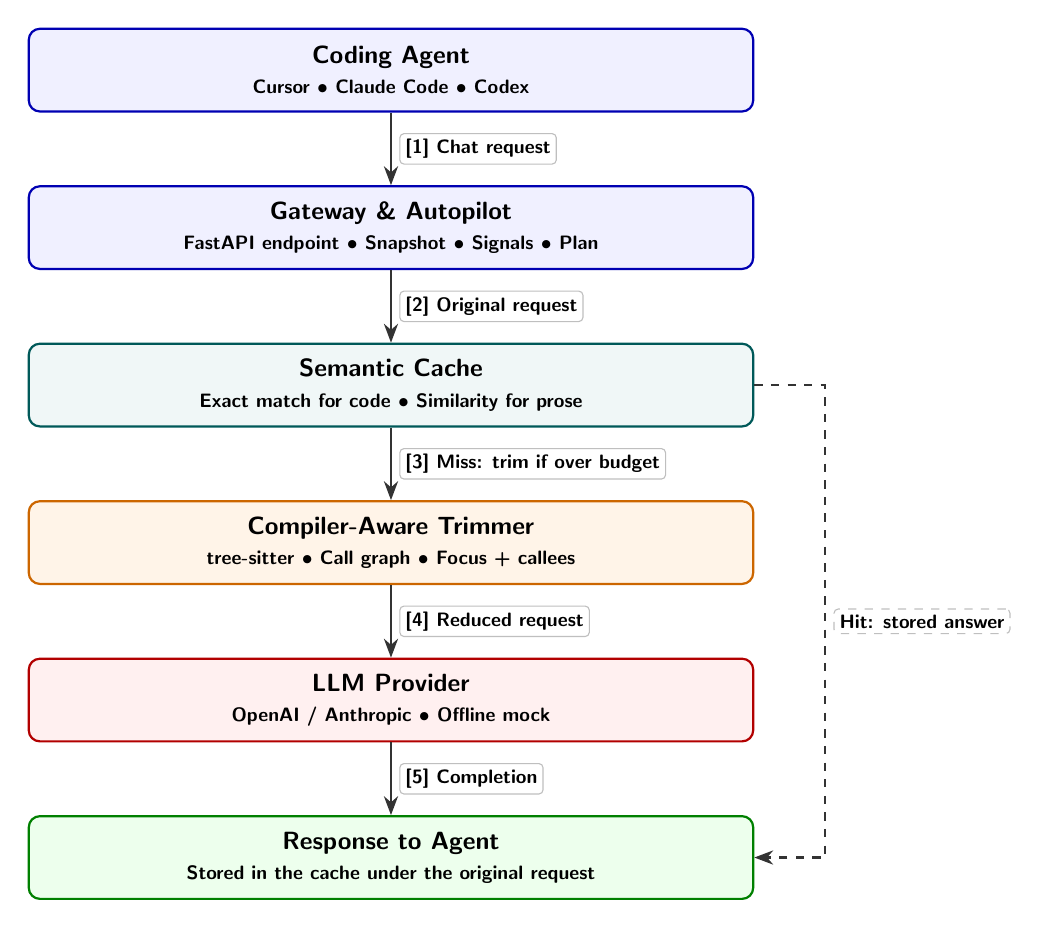
\begin{tikzpicture}[w/.style={minimum width=9.2cm, minimum height=1.05cm}]
  \node[blueb, w]   (agent) at (0,0)   {\textbf{Coding Agent}\\{\scriptsize\bfseries Cursor $\bullet$ Claude Code $\bullet$ Codex}};
  \node[blueb, w]   (gw)    at (0,-2)  {\textbf{Gateway \& Autopilot}\\{\scriptsize\bfseries FastAPI endpoint $\bullet$ Snapshot $\bullet$ Signals $\bullet$ Plan}};
  \node[tealb, w]   (cache) at (0,-4)  {\textbf{Semantic Cache}\\{\scriptsize\bfseries Exact match for code $\bullet$ Similarity for prose}};
  \node[orangeb, w] (trim)  at (0,-6)  {\textbf{Compiler-Aware Trimmer}\\{\scriptsize\bfseries tree-sitter $\bullet$ Call graph $\bullet$ Focus + callees}};
  \node[redb, w]    (llm)   at (0,-8)  {\textbf{LLM Provider}\\{\scriptsize\bfseries OpenAI / Anthropic $\bullet$ Offline mock}};
  \node[greenb, w]  (resp)  at (0,-10) {\textbf{Response to Agent}\\{\scriptsize\bfseries Stored in the cache under the original request}};
  \draw[pipe] (agent) -- node[steplbl, right=3pt] {[1] Chat request} (gw);
  \draw[pipe] (gw)    -- node[steplbl, right=3pt] {[2] Original request} (cache);
  \draw[pipe] (cache) -- node[steplbl, right=3pt] {[3] Miss: trim if over budget} (trim);
  \draw[pipe] (trim)  -- node[steplbl, right=3pt] {[4] Reduced request} (llm);
  \draw[pipe] (llm)   -- node[steplbl, right=3pt] {[5] Completion} (resp);
  \draw[pipe, dashed] (cache.east) -- ++(0.9,0) |- (resp.east)
        node[steplbl, pos=0.25, right=3pt] {Hit: stored answer};
\end{tikzpicture}
\caption{High-level request path through the gateway. On a cache hit (dashed)
the stored answer is returned and the model is never called.}
\label{fig:architecture}
\end{figure}

The three components are developed independently against interfaces frozen early
in the project (\code{gateway/interfaces.py}), so each teammate can build and test
their part with mocks. The gateway is the only place they meet.

\subsection{Design Diagrams}

The design is documented with four diagrams, all available on the project site and
in \code{docs/Diagrams/}:

\begin{itemize}
    \item \textbf{Use case diagram} (Figure~\ref{fig:usecase}): the Developer and
          the Coding Agent send requests; reducing cost is always included, while
          reusing an answer, reducing code context and calling the LLM are
          conditional extensions.
    \item \textbf{Data flow diagram} (Figure~\ref{fig:dfd}): Level~0 shows the
          gateway and its external entities, Level~1 its six processes and two data
          stores, and Level~2 the seven steps of the trimmer.
    \item \textbf{Activity (swimlane) diagram} (Figure~\ref{fig:activity}): one
          request through the gateway, with one lane per component, decisions,
          and fork/join for independent work.
    \item \textbf{ER diagram} (Figure~\ref{fig:er}): the conceptual data model,
          covering cache entries, metric records, and the trimmer's model of source
          files, functions and the calls between them.
\end{itemize}

\begin{figure}[H]
    \centering
    
\includegraphics[width=0.95\textwidth]{use-case}
    \caption{Use case diagram.}
    \label{fig:usecase}
\end{figure}

\begin{figure}[H]
    \centering
    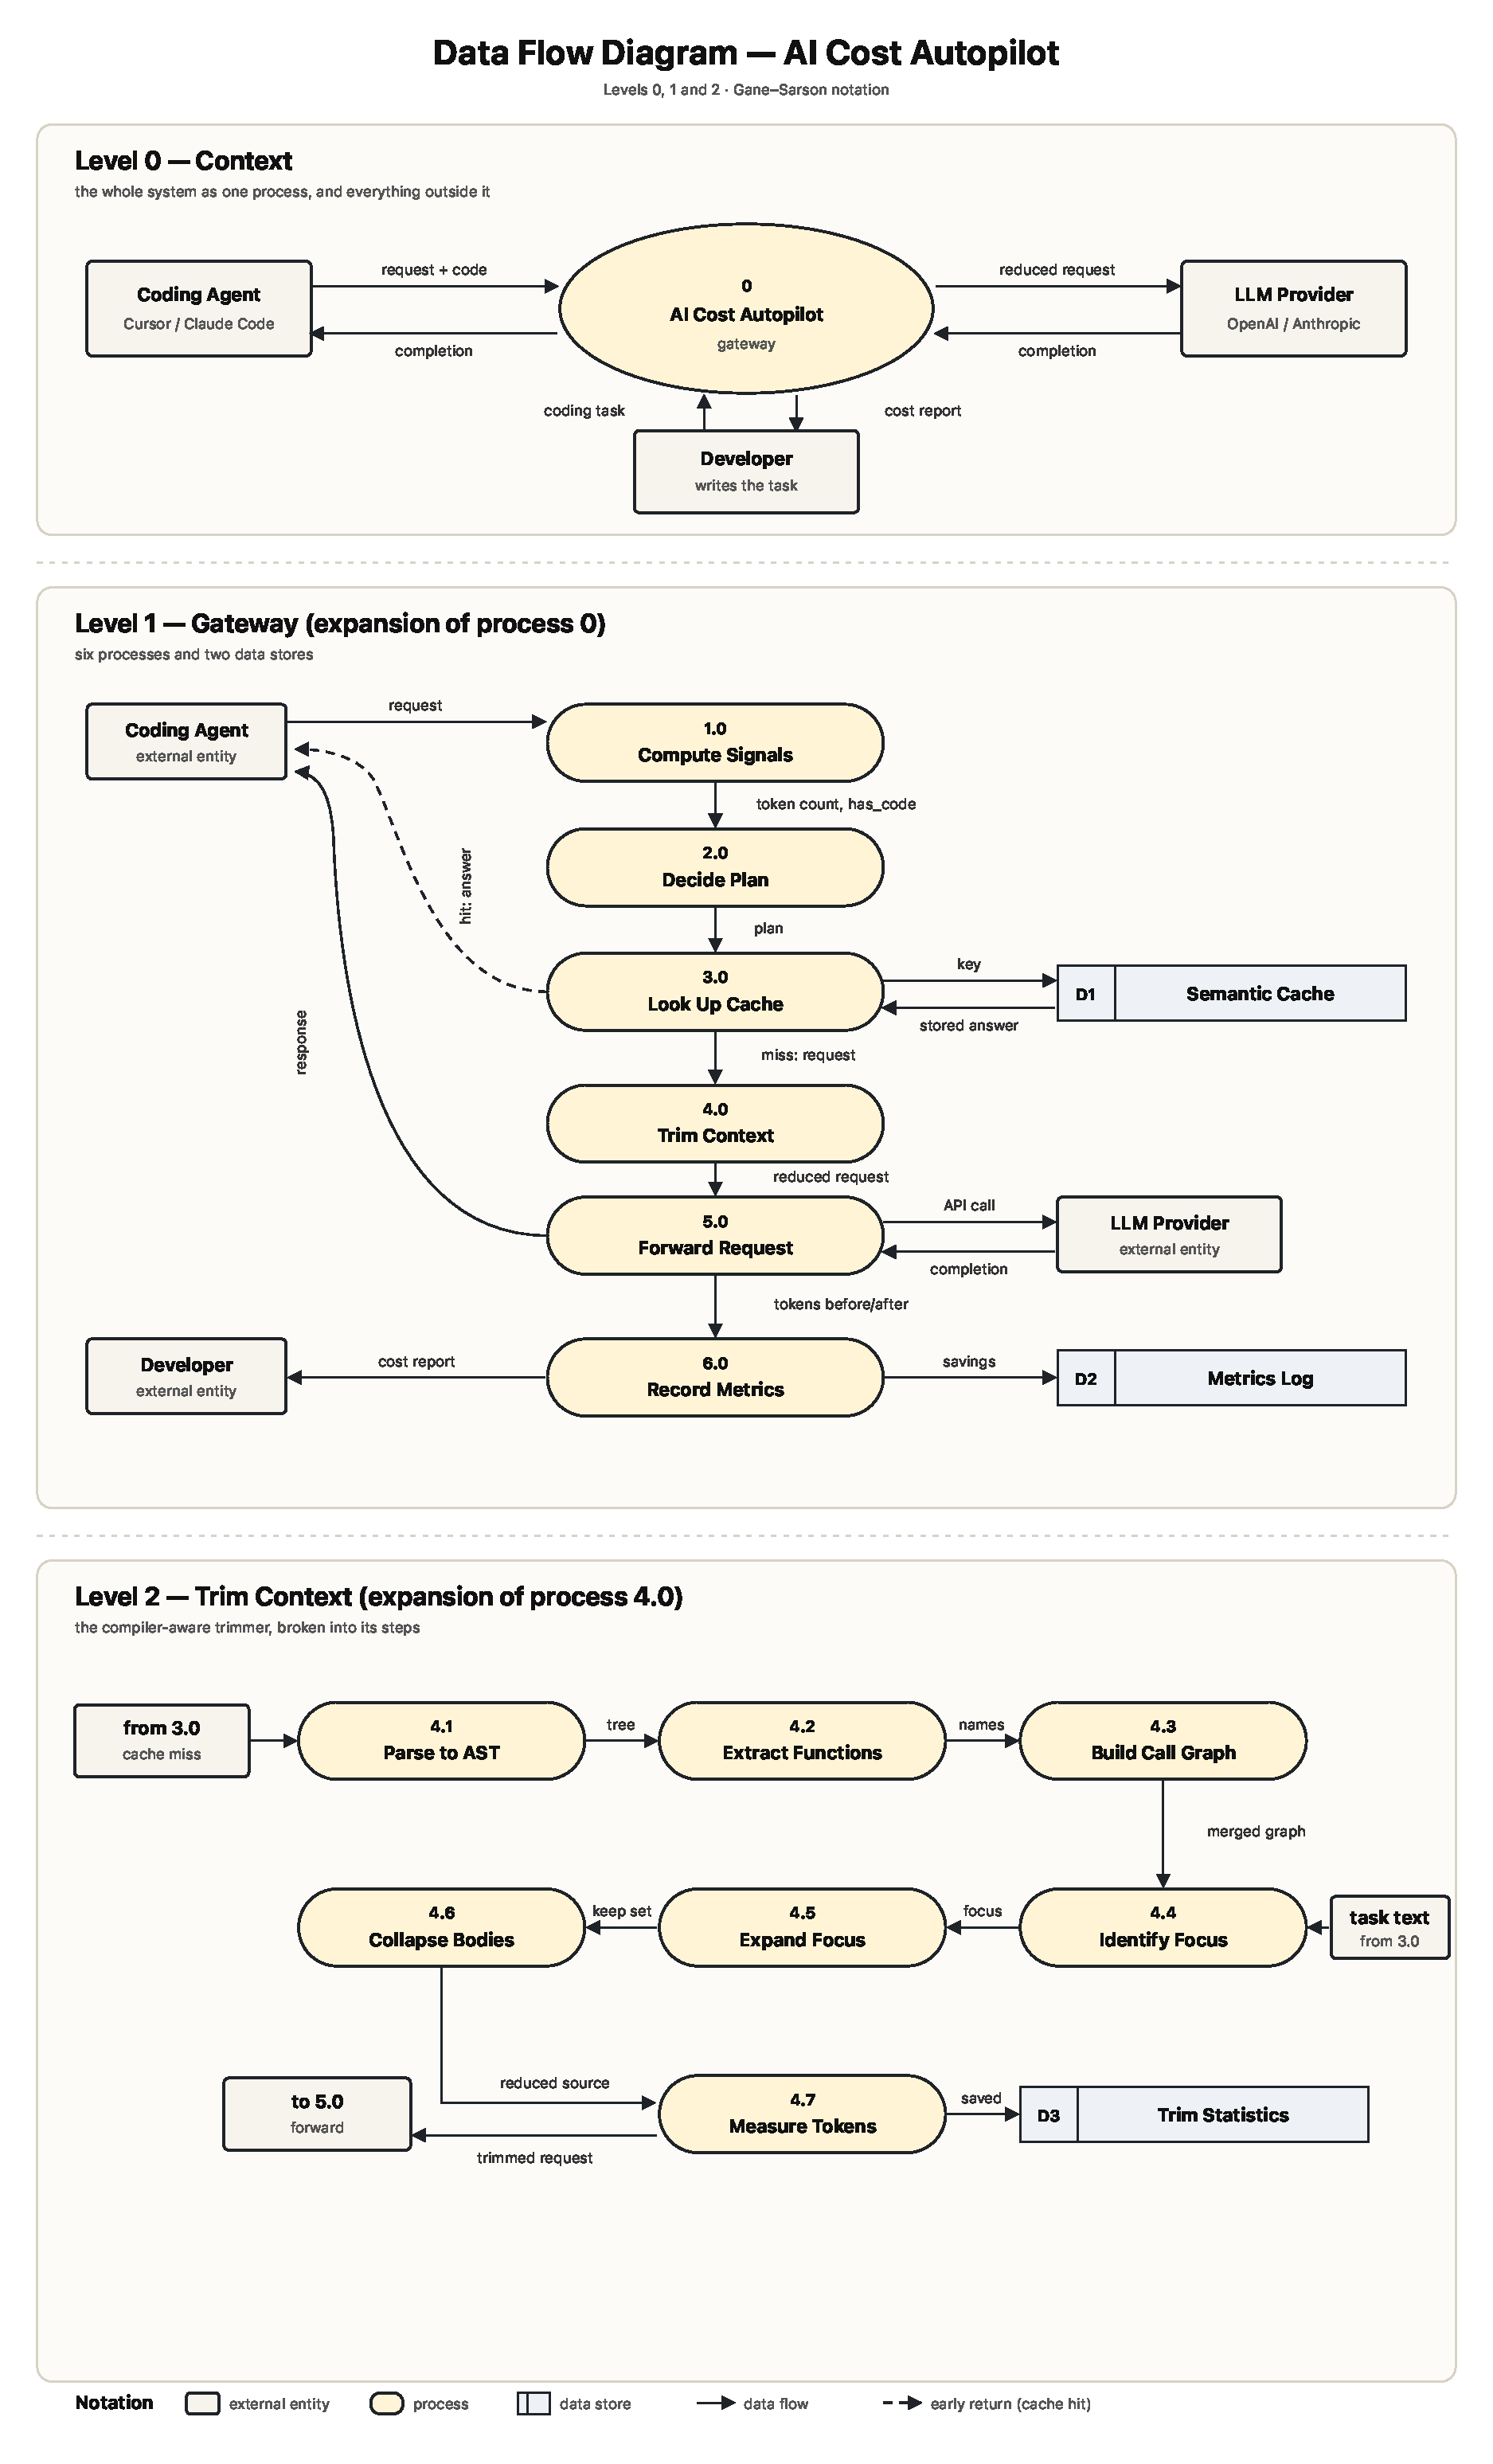
\includegraphics[height=0.82\textheight, width=\textwidth, keepaspectratio]{dfd}
    \caption{Data flow diagram, levels 0, 1 and 2.}
    \label{fig:dfd}
\end{figure}

\begin{figure}[H]
    \centering
    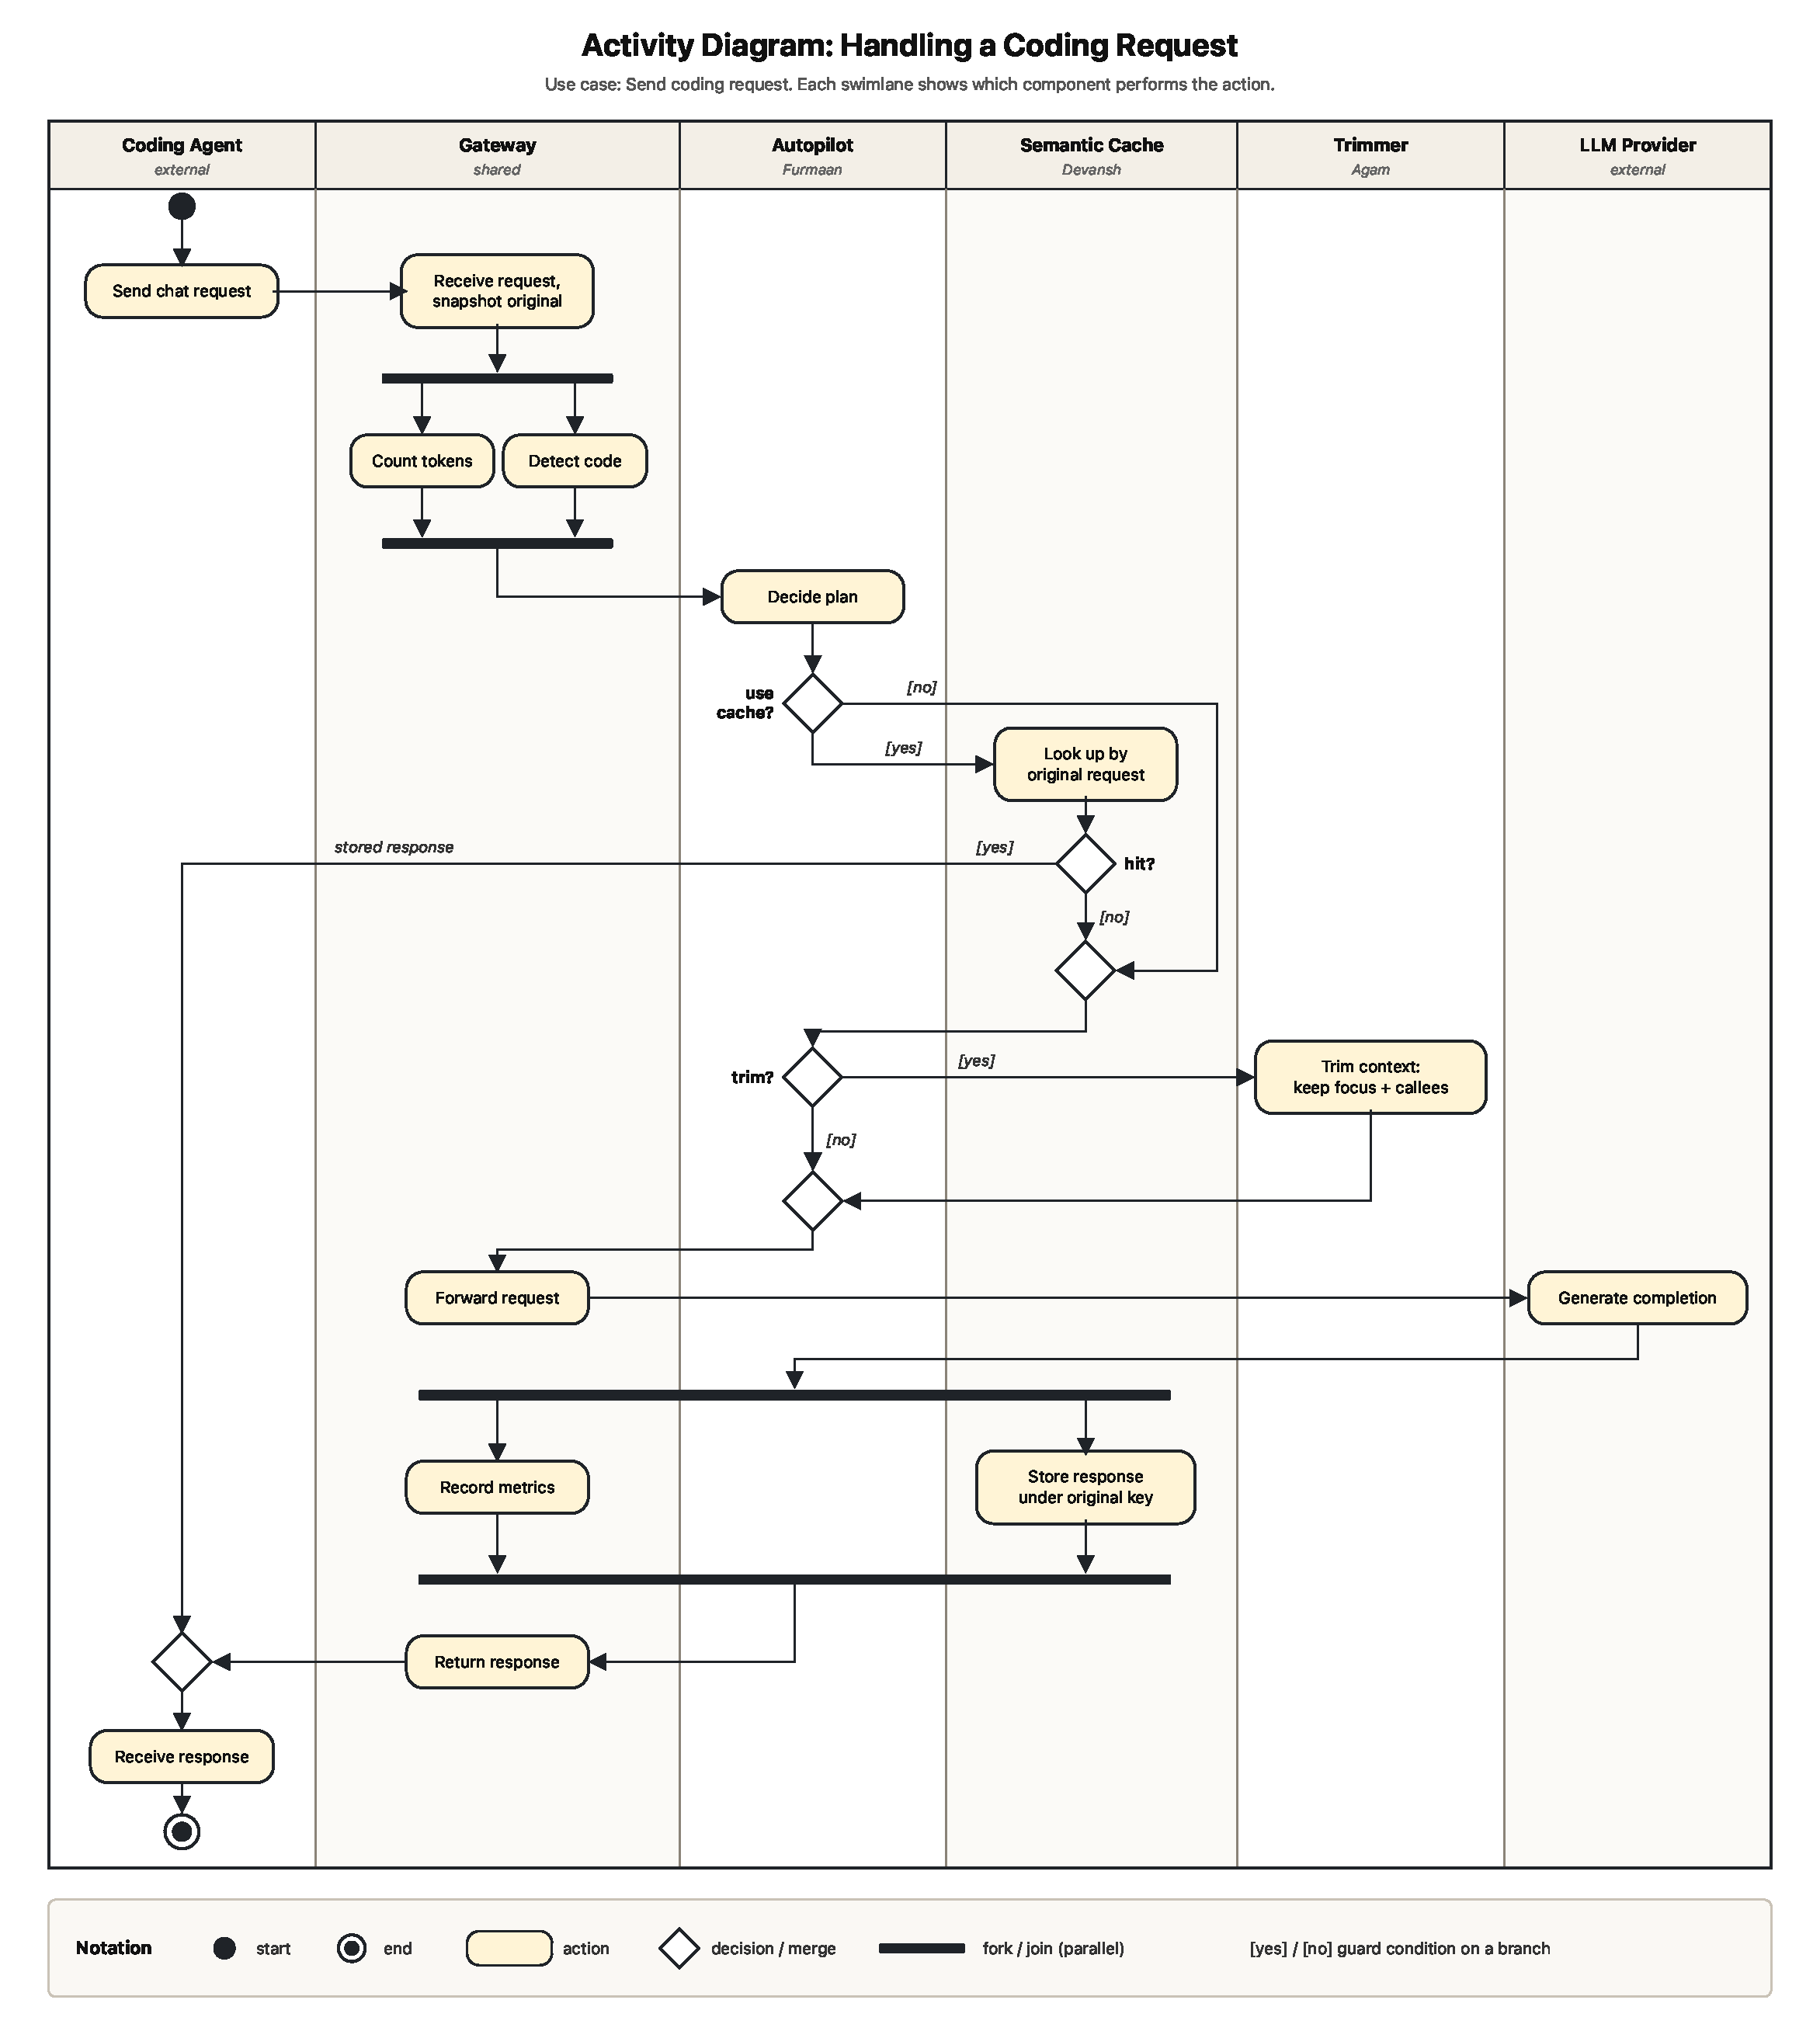
\includegraphics[height=0.82\textheight, width=\textwidth, keepaspectratio]{activity}
    \caption{Activity diagram with swimlanes for handling one coding request.}
    \label{fig:activity}
\end{figure}

\begin{figure}[H]
    \centering
    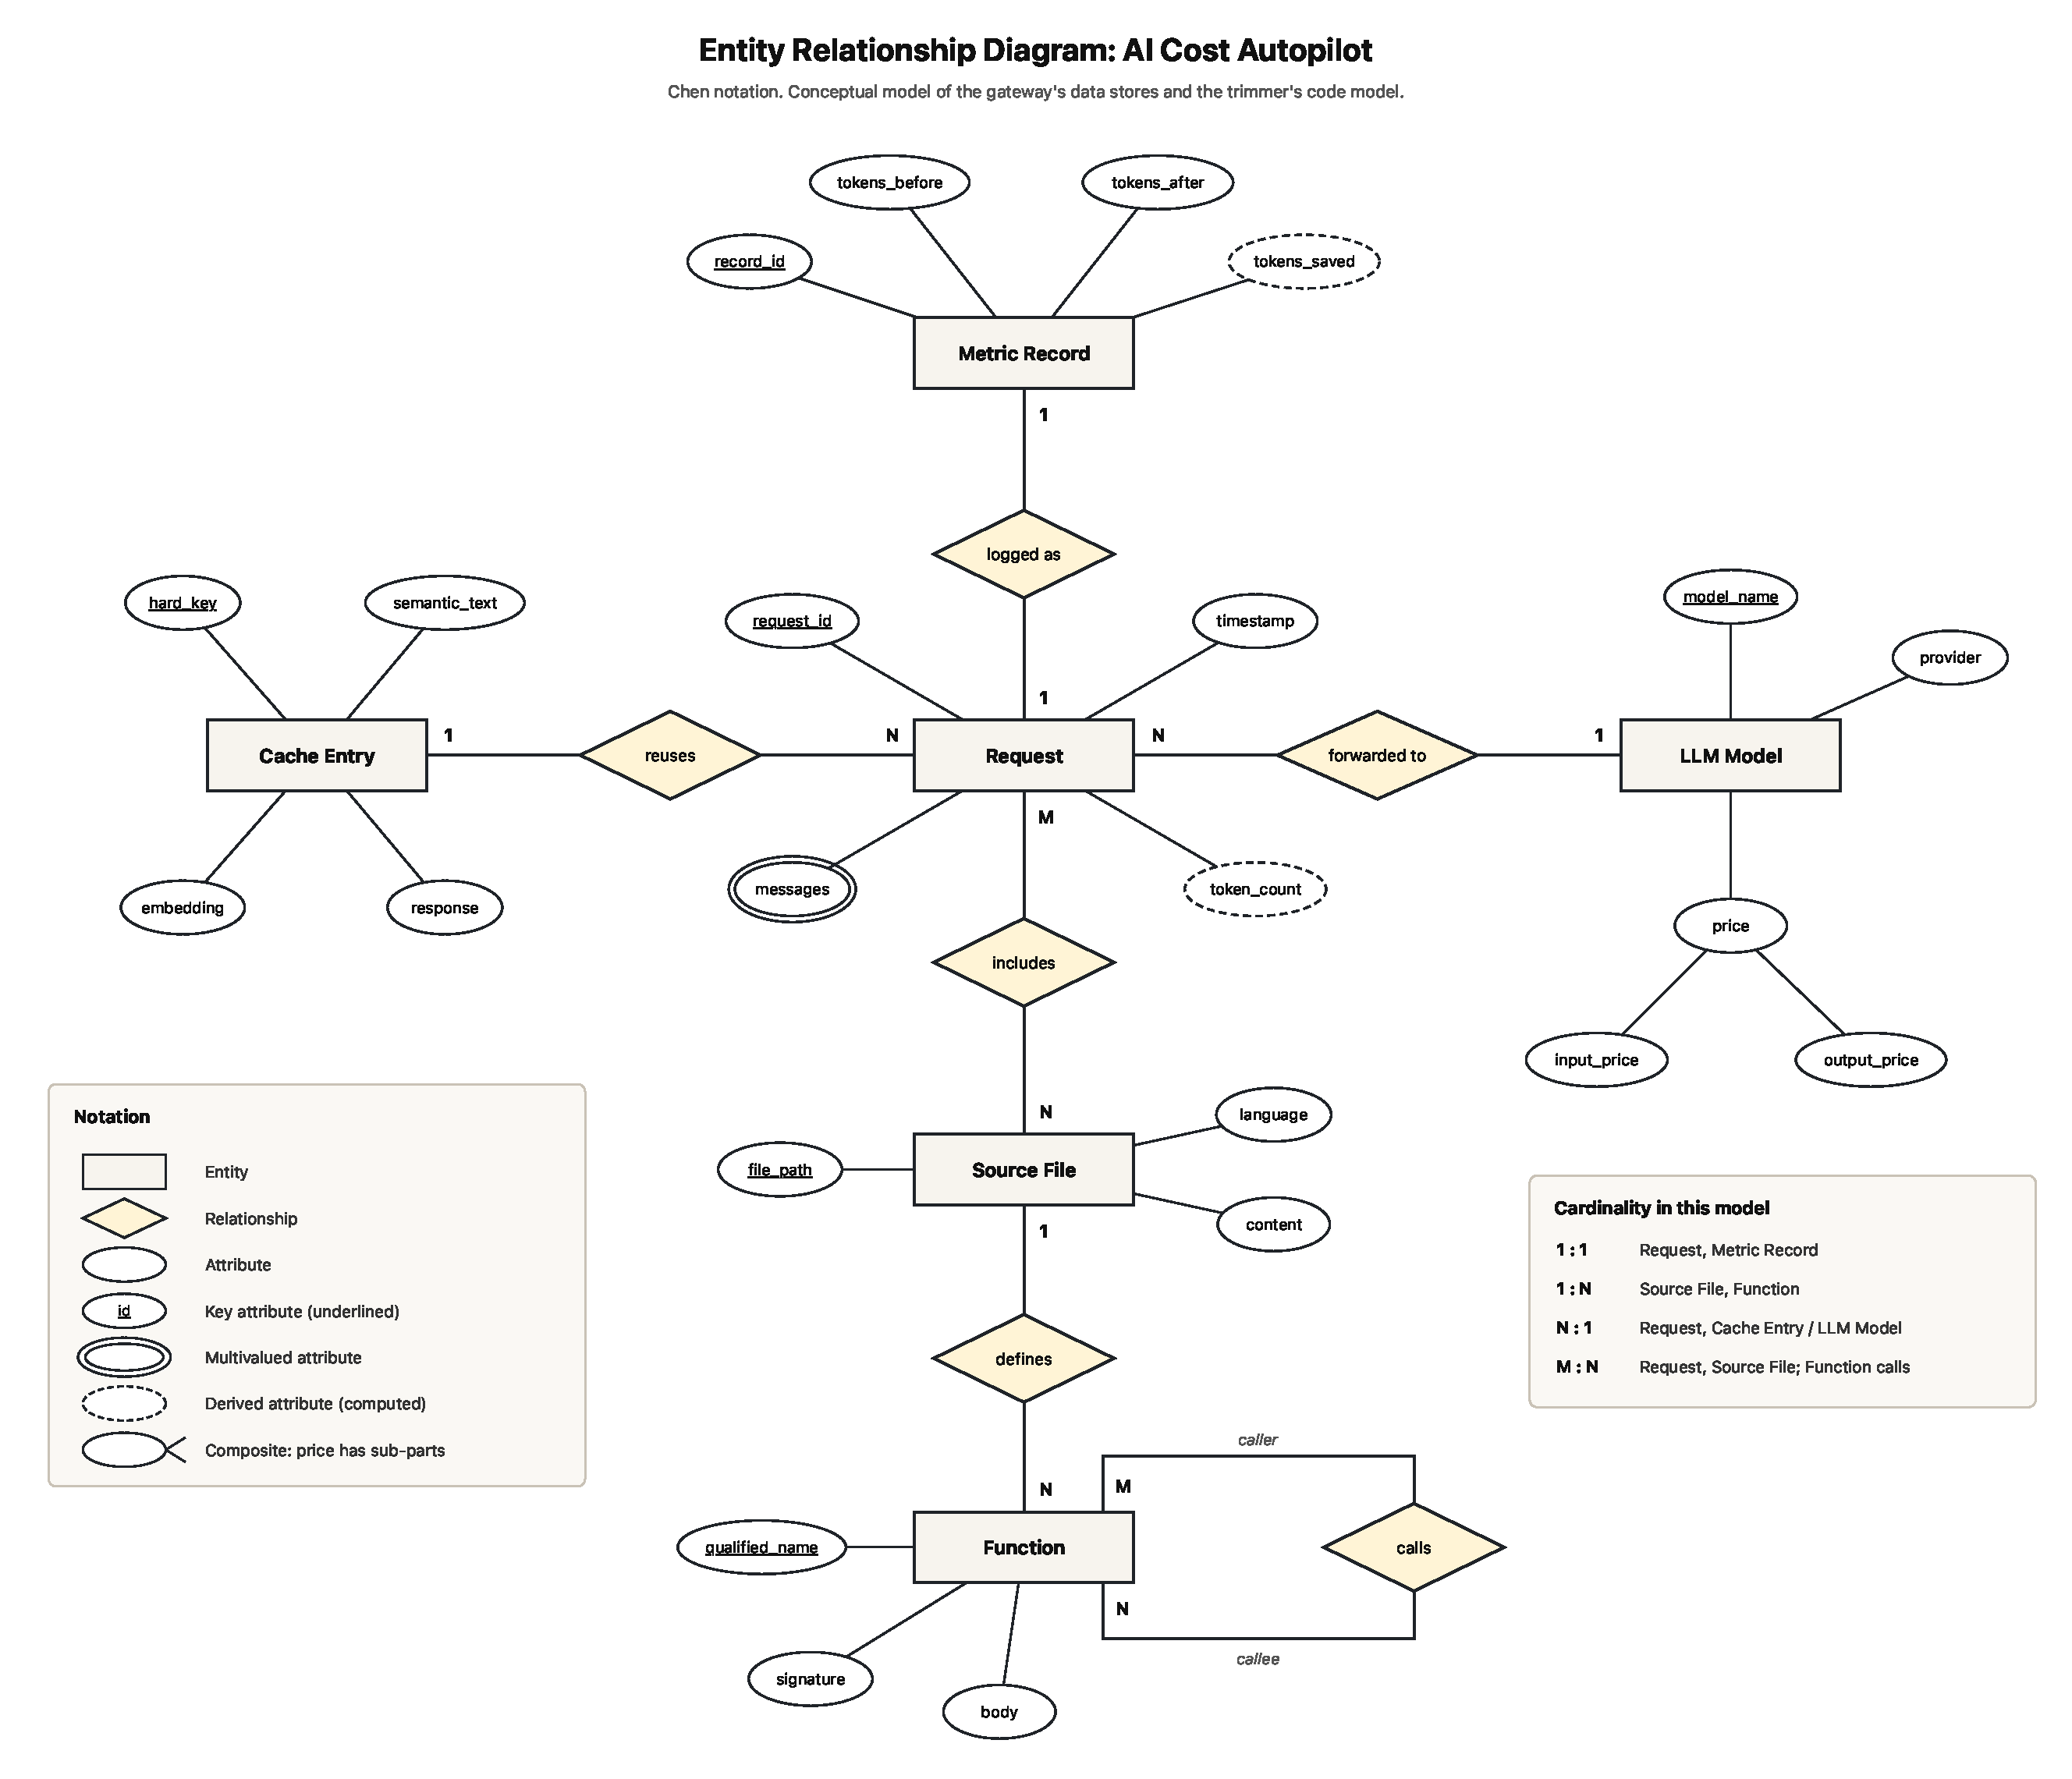
\includegraphics[width=\textwidth]{er}
    \caption{Entity relationship diagram (Chen notation).}
    \label{fig:er}
\end{figure}

\subsection{Technical Stack}

\begin{table}[H]
\centering
\begin{tabularx}{\textwidth}{>{\bfseries}l X}
\toprule
Layer & Technology \\
\midrule
Language & Python 3.12 (CI) and 3.13 (development) \\
Gateway & FastAPI, Uvicorn, httpx for forwarding \\
Parsing & tree-sitter with the \code{tree-sitter-python} grammar \\
Token counting & tiktoken, \code{cl100k\_base} encoding \\
Semantic matching & sentence-transformers, \code{all-MiniLM-L6-v2} (optional) \\
Testing and CI & pytest; GitHub Actions on every pull request and push to \code{master} \\
Documentation & MkDocs Material on GitHub Pages; LaTeX for reports \\
\bottomrule
\end{tabularx}
\caption{Technical stack.}
\end{table}

\section{Implementation Details}

\subsection{Gateway}

The gateway exposes \code{POST /v1/chat/completions} and \code{GET /health}. It
takes a deep copy of the request before anything changes it, computes the signals,
asks the autopilot for a plan, and then runs the cache, trimmer and provider in
that order. A \textbf{mock mode} returns a well-formed completion (with an id,
timestamp and estimated token usage) instead of calling a real provider. It turns
on automatically when no API key is set, so every teammate and the CI can run the
full pipeline with no key and no cost.

An early bug showed why the snapshot matters: the cache originally stored
responses \emph{after} the trimmer had rewritten the request, so a response was
filed under the trimmed text and an identical request could never hit it. Keying
both lookup and store on the original request fixed this.

\subsection{Module 1: Compiler-Aware Trimmer}

The trimmer works on the syntax tree rather than on raw text.

\begin{enumerate}
    \item \textbf{Parse.} Each code message is parsed with tree-sitter~\cite{treesitter}.
    \item \textbf{Collapse.} A function that is not needed keeps its signature and
          docstring, and its body is replaced by an ellipsis (\code{...}). Edits are applied from
          the end of the file backwards using byte offsets, so earlier positions
          stay valid and indentation is preserved. The result is always valid
          Python.
    \item \textbf{Call graph.} The trimmer records which functions each function
          calls. Calls through \code{super()} are ignored, because they go to the
          base class; treating them as calls to a same-named local function created
          false edges (for example \code{\_\_init\_\_} appearing to call itself).
          Self-edges from recursion are dropped.
    \item \textbf{Focus.} The functions the task is about are taken from names
          mentioned in the plain-text part of the request (or passed explicitly).
    \item \textbf{Expand.} A breadth-first search from the focus follows the call
          graph for up to two hops. Those functions are kept in full.
\end{enumerate}

\textbf{Cross-file dependencies.} A request usually carries one file per message.
The first version built a call graph per message, so a dependency defined in
another file was missed. On a realistic fixture, asking to ``fix
\code{create\_note}'' kept \code{create\_note} but collapsed \code{validate\_note},
which lives in a different file and is exactly what the fix needs. The trimmer now
merges one call graph across every code message in the request, resolving calls
against all functions defined anywhere in it. Figure~\ref{fig:trimmer} shows the
whole pipeline.

\begin{figure}[H]
\centering
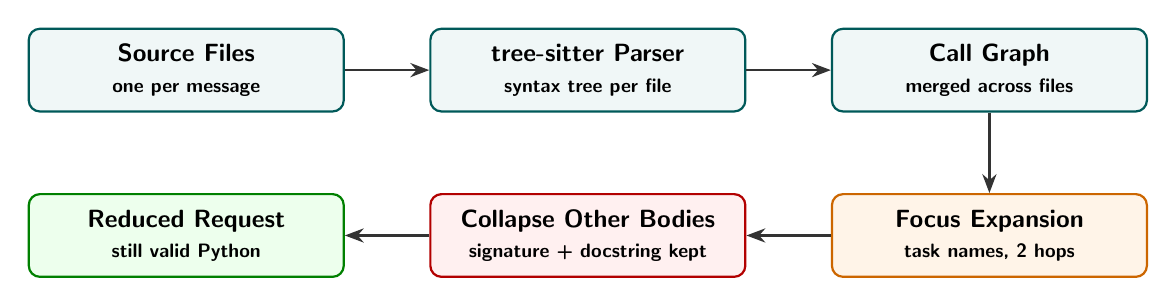
\begin{tikzpicture}[s/.style={minimum width=4.0cm, minimum height=1.05cm}]
  \node[tealb, s] (a) at (0,0)      {\textbf{Source Files}\\{\scriptsize\bfseries one per message}};
  \node[tealb, s] (b) at (5.1,0)    {\textbf{tree-sitter Parser}\\{\scriptsize\bfseries syntax tree per file}};
  \node[tealb, s] (c) at (10.2,0)   {\textbf{Call Graph}\\{\scriptsize\bfseries merged across files}};
  \node[orangeb, s] (d) at (10.2,-2.1) {\textbf{Focus Expansion}\\{\scriptsize\bfseries task names, 2 hops}};
  \node[redb, s] (e) at (5.1,-2.1)  {\textbf{Collapse Other Bodies}\\{\scriptsize\bfseries signature + docstring kept}};
  \node[greenb, s] (f) at (0,-2.1)    {\textbf{Reduced Request}\\{\scriptsize\bfseries still valid Python}};
  \draw[pipe] (a) -- (b); \draw[pipe] (b) -- (c); \draw[pipe] (c) -- (d);
  \draw[pipe] (d) -- (e); \draw[pipe] (e) -- (f);
\end{tikzpicture}
\caption{Compiler-aware trimming pipeline.}
\label{fig:trimmer}
\end{figure}

\subsection{Module 2: Semantic Cache}

Each cache entry is split into a \textbf{hard key} and the \textbf{message text}.
The hard key is a hash of everything that must match exactly: the model, every
parameter (temperature, maximum tokens, tools, response format and so on) and the
message roles. Only an explicit list of fields known not to affect the answer is
left out, so an unknown parameter makes the cache miss rather than return a wrong
answer.

Within a hard key, lookup works in three steps:
\begin{enumerate}
    \item \textbf{Exact text match}, which needs no embedding model and covers both
          code and prose.
    \item \textbf{Code is exact-only.} If the request contains code, the cache never
          reuses on similarity (see Section~\ref{sec:cache-results}).
    \item \textbf{Prose uses meaning.} For natural language, the text is embedded
          with a sentence-embedding model~\cite{sbert} and the most similar stored entry is reused if its cosine similarity is
          at least 0.90.
\end{enumerate}
Storing the same request again replaces the old entry instead of adding a
duplicate. If sentence-transformers is not installed, exact matching still works
and only similarity matching is disabled. Figure~\ref{fig:cache} shows the lookup
flow.

\begin{figure}[H]
\centering
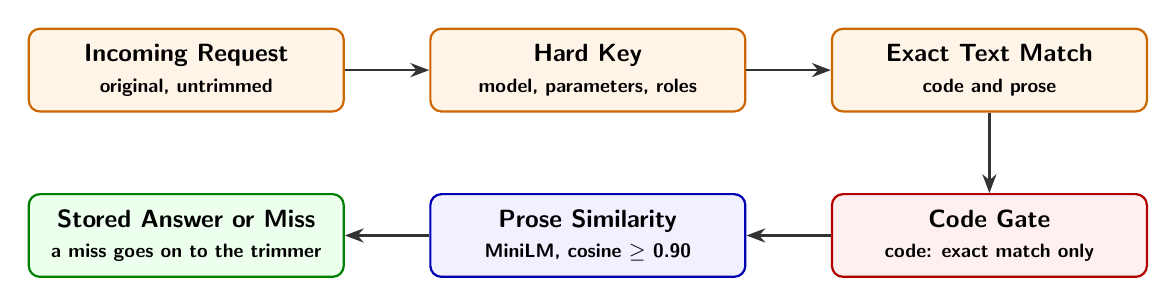
\begin{tikzpicture}[s/.style={minimum width=4.0cm, minimum height=1.05cm}]
  \node[orangeb, s] (a) at (0,0)      {\textbf{Incoming Request}\\{\scriptsize\bfseries original, untrimmed}};
  \node[orangeb, s] (b) at (5.1,0)    {\textbf{Hard Key}\\{\scriptsize\bfseries model, parameters, roles}};
  \node[orangeb, s] (c) at (10.2,0)   {\textbf{Exact Text Match}\\{\scriptsize\bfseries code and prose}};
  \node[redb, s] (d) at (10.2,-2.1) {\textbf{Code Gate}\\{\scriptsize\bfseries code: exact match only}};
  \node[blueb, s] (e) at (5.1,-2.1)  {\textbf{Prose Similarity}\\{\scriptsize\bfseries MiniLM, cosine $\geq$ 0.90}};
  \node[greenb, s] (f) at (0,-2.1)    {\textbf{Stored Answer or Miss}\\{\scriptsize\bfseries a miss goes on to the trimmer}};
  \draw[pipe] (a) -- (b); \draw[pipe] (b) -- (c); \draw[pipe] (c) -- (d);
  \draw[pipe] (d) -- (e); \draw[pipe] (e) -- (f);
\end{tikzpicture}
\caption{Semantic cache lookup flow.}
\label{fig:cache}
\end{figure}

\subsection{Module 3: Autopilot}

The autopilot turns the signals into a plan, in order of cost. First, a
\textbf{safety check}: if the request contains a secret it is never cached,
neither read from the cache nor written to it. The scan covers API keys in their
current formats (OpenAI \code{sk-proj-}, Anthropic \code{sk-ant-}, Google, GitHub,
AWS), private keys, tokens, and quoted password or key literals, and it reads
multipart messages as well as plain text. It deliberately ignores ordinary code
such as \code{password = payload.get("password")}, which would otherwise switch
off caching for any code that handles logins. Second, the cache is always tried.
Third, trimming is requested when the request contains code and is estimated at
over 1000 tokens; a secret does not stop trimming, because trimming caches nothing
and sends less code to the provider. The autopilot also counts its decisions, as
the basis for tuning its thresholds later.

The trimmer applies its own 8000-token budget on top of the autopilot's
1000-token threshold, so for requests in between the plan asks for trimming that
does not happen. Aligning the two thresholds is next-stage work.

\section{Development Process}

Work happens on feature branches. Every change to \code{master} goes through a pull
request that needs one approving review from a teammate, and the GitHub Actions
test workflow runs on every pull request and on
every push to \code{master}. Reviews have caught real defects in both
directions: missing parameters in the cache key and a cache that returned the
oldest duplicate were found in review, as was the trimmed-key bug described above.
Each member keeps a weekly technical journal in the repository.

% =========================================================================
% CHAPTER 3: RESULTS AND EVALUATION
% =========================================================================
\chapter{Results and Evaluation}

\section{Testing Methodology}

The test suite has 65 tests: 24 for the trimmer, 21 for the cache, 13 for the
autopilot and 7 for the gateway, most of which send real HTTP requests through the
whole pipeline using the mock provider. At the time of writing, 64 pass and 1 is skipped
(the test that needs the real embedding model, which is not installed in CI).
Figure~\ref{fig:testing} shows how the suites feed continuous integration.

\begin{figure}[H]
\centering
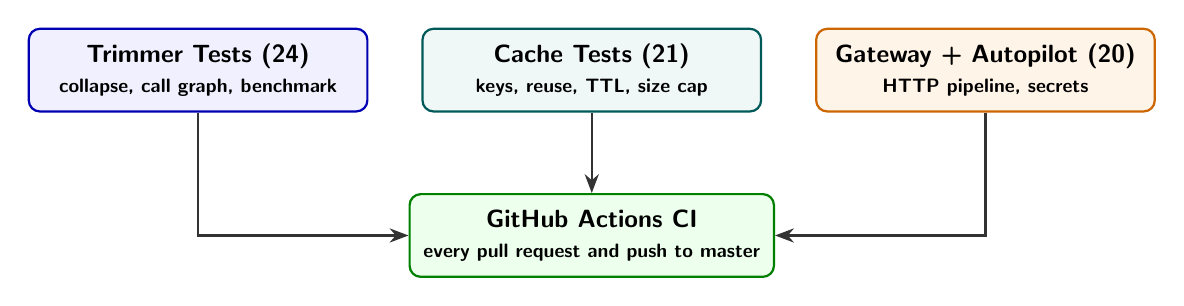
\begin{tikzpicture}[t/.style={minimum width=4.3cm, minimum height=1.05cm}]
  \node[blueb, t]   (u) at (0,0)     {\textbf{Trimmer Tests (24)}\\{\scriptsize\bfseries collapse, call graph, benchmark}};
  \node[tealb, t]   (c) at (5.0,0)   {\textbf{Cache Tests (21)}\\{\scriptsize\bfseries keys, reuse, TTL, size cap}};
  \node[orangeb, t] (g) at (10.0,0)  {\textbf{Gateway + Autopilot (20)}\\{\scriptsize\bfseries HTTP pipeline, secrets}};
  \node[greenb, t]  (ci) at (5.0,-2.1) {\textbf{GitHub Actions CI}\\{\scriptsize\bfseries every pull request and push to master}};
  \draw[pipe] (u.south) |- (ci.west);
  \draw[pipe] (c.south) -- (ci.north);
  \draw[pipe] (g.south) |- (ci.east);
\end{tikzpicture}
\caption{Test suites and continuous integration.}
\label{fig:testing}
\end{figure}

Measurements use a realistic fixture, \code{notes\_api}: a small but genuine
service with 10 files, 45 functions and 3,277 tokens, with real imports between
files. A toy project of two files was not enough, because in a project that small
almost every function is reachable from every other, so there is nothing to trim
selectively. Every file in the fixture is checked to compile, and tokens are
counted with tiktoken~\cite{tiktoken} (\code{cl100k\_base}).

\section{Performance Metrics}

\subsection{Trimmer against simple baselines}

Table~\ref{tab:trimmer} compares the trimmer with simpler ways of shrinking the
same request, for the task ``fix \code{create\_note}''. Every variant is measured
on the same file contents, and ``valid'' means every output file still compiles
as Python. The table is produced by \code{python -m trimmer.benchmark.baselines},
and CI checks the relationships it shows.

\begin{table}[H]
\centering
\begin{tabular}{lrrl}
\toprule
Variant & Tokens & Saved & Output \\
\midrule
Raw request (no gateway)                         & 3,277 & --      & valid \\
Strip indentation and blank lines                & 2,982 & 9.0\%  & \textbf{broken} \\
Strip comments and docstrings                    & 2,606 & 20.5\% & valid \\
Collapse every function body                     & 1,410 & 57.0\% & valid, but drops the focus \\
\textbf{Trimmer (focus and callees, 2 hops)}     & \textbf{2,166} & \textbf{33.9\%} & \textbf{valid} \\
\bottomrule
\end{tabular}
\caption{Token reduction on the \code{notes\_api} fixture.}
\label{tab:trimmer}
\end{table}

The trimmer kept 18 of the 45 functions in full, including \code{validate\_note}
from another file, and collapsed the other 27 to their signatures. ``Fix
\code{create\_note}'' is the hardest task on this fixture because it is the most
connected function; on three other tasks the trimmer saves between 47\% and 55\%.

\subsection{Cache: can similarity be trusted for code?}
\label{sec:cache-results}

We scored labelled pairs of requests with the embedding model. A safe threshold
needs every same-meaning pair above it and every different-meaning pair below it.

\begin{table}[H]
\centering
\begin{tabular}{lr}
\toprule
Group & Cosine similarity \\
\midrule
Same meaning (should reuse)          & 0.881 -- 1.000 \\
Different meaning (must not reuse)   & 0.609 -- 0.985 \\
\midrule
\code{return a and b} vs \code{return a or b} & 0.985 \\
\code{xs[:n]} vs \code{xs[:n-1]}               & 0.972 \\
\code{a > b} vs \code{a >= b}                  & 0.956 \\
\bottomrule
\end{tabular}
\caption{Similarity ranges for code pairs.}
\label{tab:threshold}
\end{table}

The ranges overlap, and code that means the opposite scores near the top. The
only threshold with no wrong reuse (0.99) misses four of five genuine reuses. For
prose the groups separate cleanly (0.978 against 0.609), which is why the cache
uses similarity for prose only and exact matching for code.

\subsection{Cache: savings depend on repetition}

The cache savings benchmark (\code{cache/benchmark/savings.py}) replays sessions
of 20 requests through the gateway logic, varying how many requests repeat an
earlier one exactly, and averages 25 seeded sessions per repeat rate
(Table~\ref{tab:repeat}).

\begin{table}[H]
\centering
\begin{tabular}{rr}
\toprule
Requests that are repeats & Input tokens saved \\
\midrule
0\%  & 0.0\% \\
20\% & 21.2\% \\
40\% & 38.6\% \\
50\% & 49.4\% \\
60\% & 53.2\% \\
80\% & 74.4\% \\
\bottomrule
\end{tabular}
\caption{Cache savings against the share of repeated requests.}
\label{tab:repeat}
\end{table}

\subsection{Cache: added latency}

The latency benchmark (\code{cache/benchmark/latency.py}, median of 200 runs, with
the embedding model installed) measures the time the cache adds to a request
(Table~\ref{tab:latency}). Exact matches, which include every code request, cost
almost nothing. Only prose that is not an exact repeat pays for an embedding, and
a miss pays twice, once in the lookup and once when the answer is stored.

\begin{table}[H]
\centering
\begin{tabular}{lr}
\toprule
Case & Added latency \\
\midrule
Hit, exact repeat or code (no embedding)    & about 0.003 ms \\
Hit, prose paraphrase (one embedding)       & about 4.6 ms \\
Miss, prose (lookup and store, two embeddings) & about 8.4 ms \\
Cold start (one-time model load)            & about 7.5 s \\
\bottomrule
\end{tabular}
\caption{Latency added by the cache.}
\label{tab:latency}
\end{table}

\subsection{Autopilot: secret detection}

Against 4,000 randomly generated keys in the current OpenAI (\code{sk-proj-}) and
Anthropic (\code{sk-ant-}) formats, the secret scan missed none. It does not flag
the \code{notes\_api} fixture, ordinary authentication code, or kebab-case text,
so it does not switch off savings on normal requests.

\subsection{End-to-end demonstration}

The demo script (\code{python demo.py}) replays a scripted session of six requests
through the real gateway with the mock provider. The gateway sent 7,309 of 19,824
tokens (63\% fewer): 9,916 tokens were saved by cache hits and 2,599 by trimming a
large file, and every request was answered. This figure depends on the script,
which repeats a large request, so it illustrates the pipeline rather than
predicting savings on other workloads.

\section{Analysis}

\begin{itemize}
    \item \textbf{The trimmer beats text stripping and stays correct.} Stripping
          comments and docstrings, the simplest safe change, saves 20.5\%. The
          trimmer saves 33.9\% while keeping everything the task depends on.
          Removing indentation looks like a cheap win but produces broken Python.
    \item \textbf{Correctness costs savings, and that is the right trade.} Before
          the cross-file fix, the trimmer saved 53.8\% on the same task, but only
          because it collapsed \code{validate\_note}, which the fix needed. The
          realistic fixture is what exposed this; the toy project could not.
          Collapsing every body saves 57.0\% for the same reason: it throws away
          the code being fixed.
    \item \textbf{Cache savings are set by the workload.} Savings track the share
          of repeated requests almost exactly, so a single ``percent saved'' figure
          says more about the chosen workload than about the cache. We therefore
          report the curve.
    \item \textbf{Whole-request caching rarely hits in multi-turn sessions.} An
          agent resends the whole conversation each turn, and the history grows,
          so the full request is almost never repeated exactly. In our test, the
          same question asked again on the third turn of a conversation did not
          hit. This limits the cache on real agent traffic.
    \item \textbf{The token budget decides whether the trimmer runs.} The trimmer
          only acts above the 8000-token budget. The \code{notes\_api} request
          (3,277 tokens) is below it, so the measurements above set the budget
          explicitly. The autopilot asks for trimming above 1000 estimated
          tokens, so the two thresholds disagree; choosing one budget is part of
          the next stage.
\end{itemize}

% =========================================================================
% CHAPTER 4: CONCLUSION
% =========================================================================
\chapter{Conclusion}

\section{Summary of Work}

The prototype runs end to end: an OpenAI-compatible gateway with a mock provider,
a compiler-aware trimmer for Python that follows dependencies across files, a
cache that reuses exact repeats and prose paraphrases while refusing similarity
matches for code, and an autopilot that never caches secrets. It has 65 automated tests running in
CI, design documentation on the project site, and a realistic fixture for
measurement.

\section{Key Findings}

\begin{enumerate}
    \item On a realistic request, the trimmer cuts 33.9\% of tokens and the output
          is always valid code, against 20.5\% for the best simple safe baseline.
    \item A realistic fixture is essential: it exposed a dependency bug that had
          been inflating the trimmer's savings.
    \item No cosine threshold separates same-meaning from different-meaning code
          with a general-purpose embedding model, so code must use exact matching.
    \item Cache savings equal the repetition rate of the workload, and whole-request
          matching rarely hits in multi-turn sessions.
\end{enumerate}

\section{Limitations}

\begin{itemize}
    \item Only Python is supported.
    \item The autopilot's thresholds are fixed; tuning them from measured
          savings is not built yet, and its trim threshold is not yet aligned
          with the trimmer's budget.
    \item Metrics (DFD process 6.0) are designed but not yet stored by the gateway.
    \item Calls to a class, such as \code{raise ConfigError(...)}, do not yet
          create call-graph edges, so the class's constructor can be collapsed.
    \item The trimmer's savings are measured on one fixture (four tasks) so far.
\end{itemize}

\section{Future Work and Recommendations}

\begin{itemize}
    \item A reproducible ablation benchmark (raw, trimmer only, cache only, both)
          across several tasks and fixtures, and a principled choice of token
          budget.
    \item A second language (TypeScript) for the trimmer.
    \item Autopilot threshold tuning from measured savings, with one shared trim threshold.
    \item A metrics store and a savings report for developers.
    \item For multi-turn traffic, caching at the level of the conversation prefix
          rather than the whole request, and evaluating a code-aware embedding model.
    \item A benchmark across at least two coding agents through one endpoint.
\end{itemize}

\section{Final Remarks}

The prototype shows that a gateway which understands code structure can reduce what
a coding agent sends without breaking it, and it gives us honest baselines to
measure every later improvement against. The measurements also changed our plans:
they showed where the easy percentage figures were misleading, and where the next
real gains are.

\begin{thebibliography}{9}
\bibitem{databricks} Databricks, ``Managing AI coding costs at scale,'' Databricks
    Blog. \url{https://www.databricks.com/blog/managing-ai-coding-costs-scale}
\bibitem{treesitter} Tree-sitter, an incremental parsing system.
    \url{https://tree-sitter.github.io/tree-sitter/}
\bibitem{tiktoken} OpenAI, \emph{tiktoken}: a fast BPE tokeniser.
    \url{https://github.com/openai/tiktoken}
\bibitem{sbert} N.~Reimers and I.~Gurevych, ``Sentence-BERT: Sentence Embeddings
    using Siamese BERT-Networks,'' \emph{EMNLP}, 2019.
\end{thebibliography}

\end{document}
